\newpage % orphaned line.

\section{Clasificación} \label{chapter-implementacion:clasificacion}

\paragraph{} En lo que respecta a la clasificación, se implementó un componente encargado de clasificar un conjunto de ejemplos de validación dado uno o más clasificadores ya entrenados.
Llevar a cabo esta implementación fue necesario dado que por restricciones de los recursos disponibles, evaluar el rendimiento de los clasificadores construidos mediante validación cruzada insumía una gran cantidad tiempo, limitando la agilidad del desarrollo.
Como consecuencia, se consideró como alternativa válida separar un conjunto de datos de validación a clasificar con este módulo, con el fin de obtener métricas de rendimiento de esta manera. 

\paragraph{} El componente implementado, además de disponibilizar las funcionalidades descritas anteriormente, proporciona métricas de interés adicionales.
Dentro de las métricas calculadas se encuentran el makespan esperado y el obtenido mediante predicciones.
Estas métricas son consideradas como fundamentales para evaluar el rendimiento de los clasificadores, dado que de manera independiente a la precisión, es necesario evaluar la métrica fundamental asociada al éxito de una solución del problema HCSP, que como se explica en la sección \ref{section:descripcion-problema,subsection:estimacion-tiempo-ejecucion}, es el tiempo insumido por la máquina que finaliza su ejecución por último.
Con estos dos valores se puede evaluar qué tan exitosa fue la planificación obtenida mediante el uso de clasificadores en comparación con la solución obtenida mediante la heurística de referencia.
Finalmente, se calcula el porcentaje de ocasiones en las que el clasificador, al predecir erróneamente, escoge una máquina más rápida (constituyendo una acción ávida).
Esta métrica se calcula con el fin de evaluar si un clasificador se alejó de lo esperado en términos de precisión y makespan por haber aprendido a comportarse de manera ávida y por lo tanto aprendiendo a maximizar el beneficio local para cada tarea.

\paragraph{} La implementación de el componente de clasificación consta fundamentalmente de scripts, y la Figura \ref{fig:diagrama-clasificacion} presenta un diagrama de secuencia que explicita su funcionamiento.

\newpage % orphaned line.

\paragraph{} En la implementación, inicialmente se invoca el script encargado de realizar todo este análisis sobre un conjunto de ejemplos de validación.
Estos ejemplos de validación deben estar presentes en un directorio especificado mediante opciones al invocar el script.
Posteriormente, el script invoca al script de clasificación sobre cada uno de los ejemplos de validación encontrados.
El script de clasificación se encarga de cargar el clasificador a utilizar desde una ubicación especificada del sistema de archivos.
Una vez que todas las instancias de validación se encuentran clasificadas, se efectúa el cálculo de métricas en el script de análisis.
Finalmente, el resultado es devuelto al usuario.

\textsc{\begin{figure}[ht!]
	\centering
    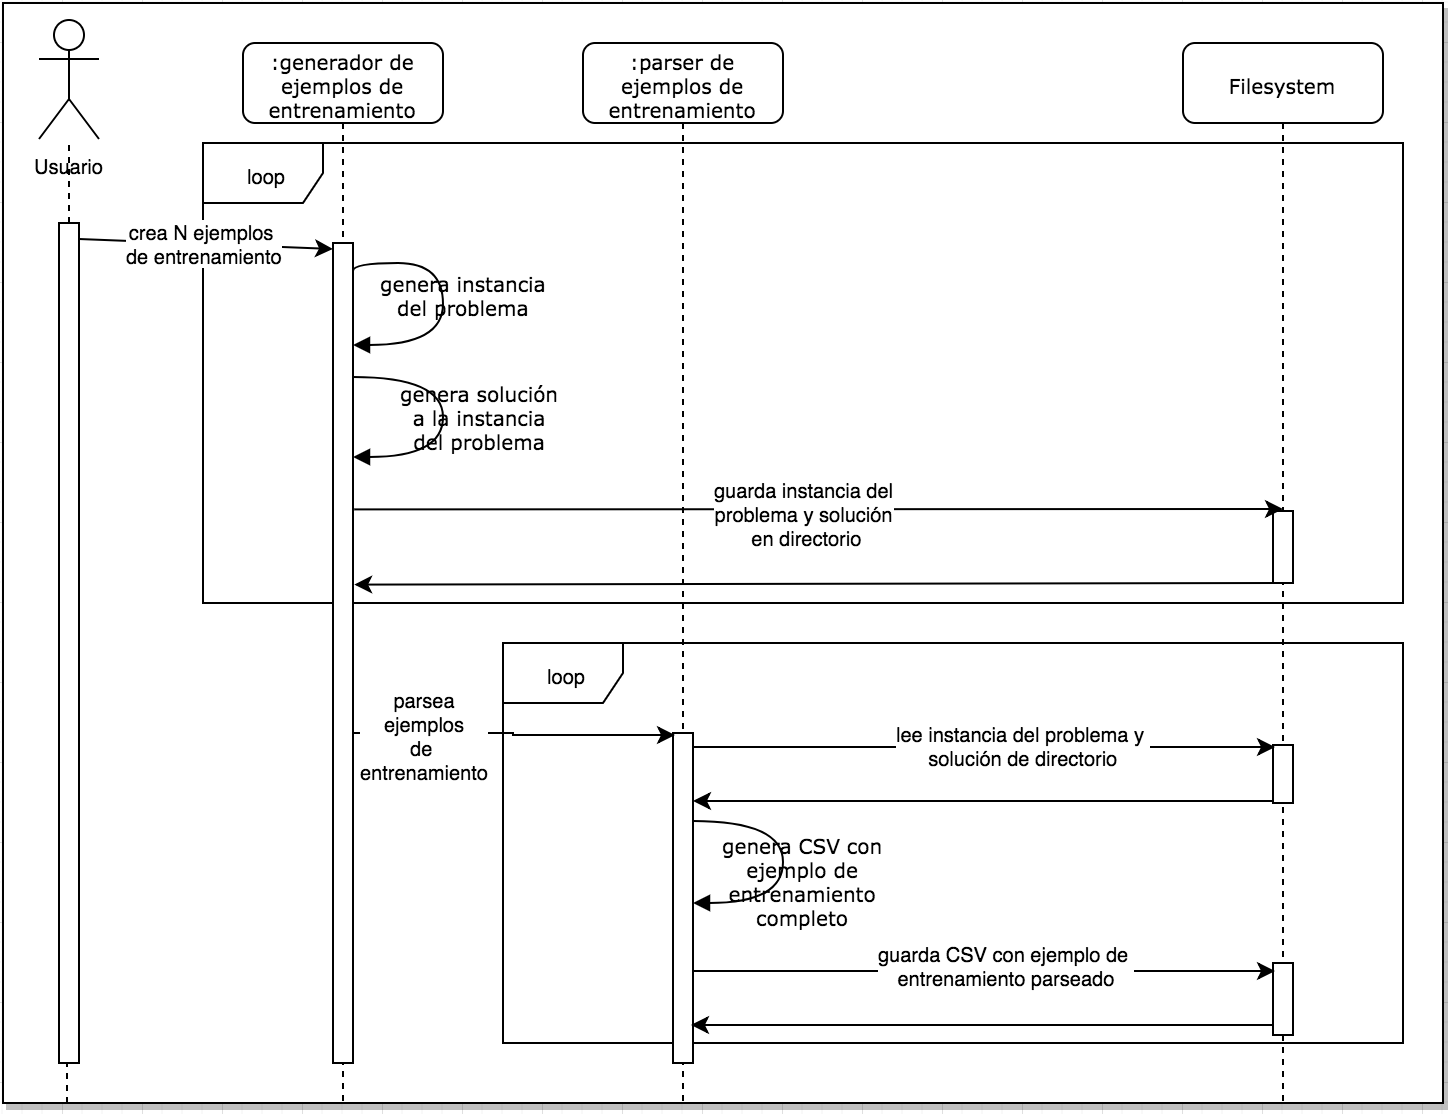
\includegraphics[width=.9\linewidth]{imagenes/implementacion/diagrama-datos.png} % TODO cambiar por validation
	\caption{Diagrama de secuencia de clasificación de ejemplos de validación.}
	\label{fig:diagrama-clasificacion}
\end{figure}}



